\begin{figure}[H]
  \centering
  \captionsetup{justification=centering}

  % Fila 1
  \begin{subfigure}[b]{0.495\textwidth}
    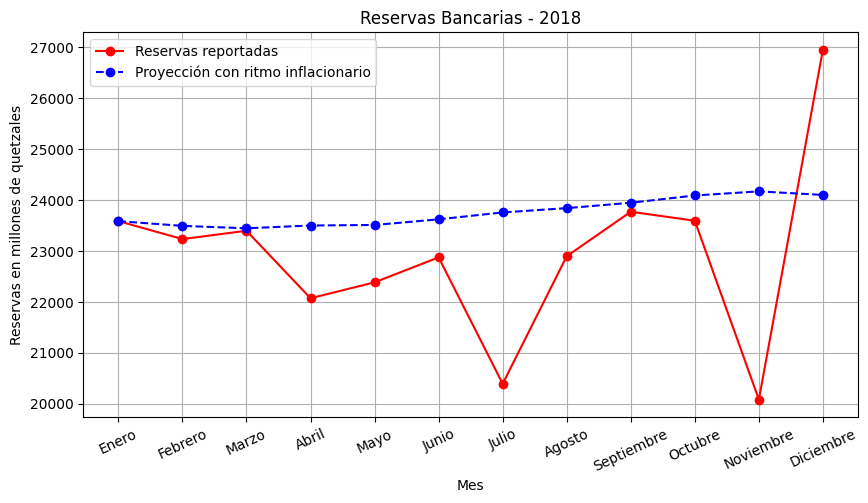
\includegraphics[width=\linewidth]{imagenes/reservas_2018.png}
    \caption{2018}
    \label{proyeccion reservas inicio de año}
  \end{subfigure}
  % No hay espacio intencionalmente entre las figuras para maximizar el tamaño de la imagen
  \begin{subfigure}[b]{0.495\textwidth}
    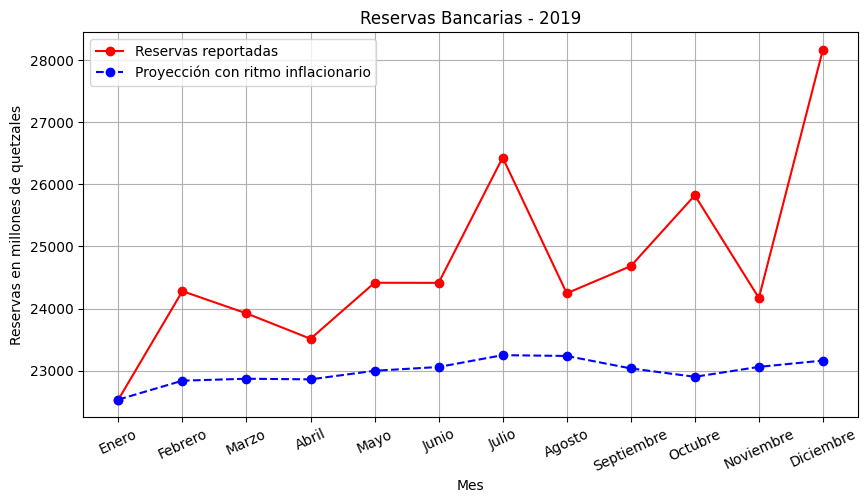
\includegraphics[width=\linewidth]{imagenes/reservas_2019.png}
    \caption{2019}
  \end{subfigure}
  
  % Fila 2
  \begin{subfigure}[b]{0.495\textwidth}
    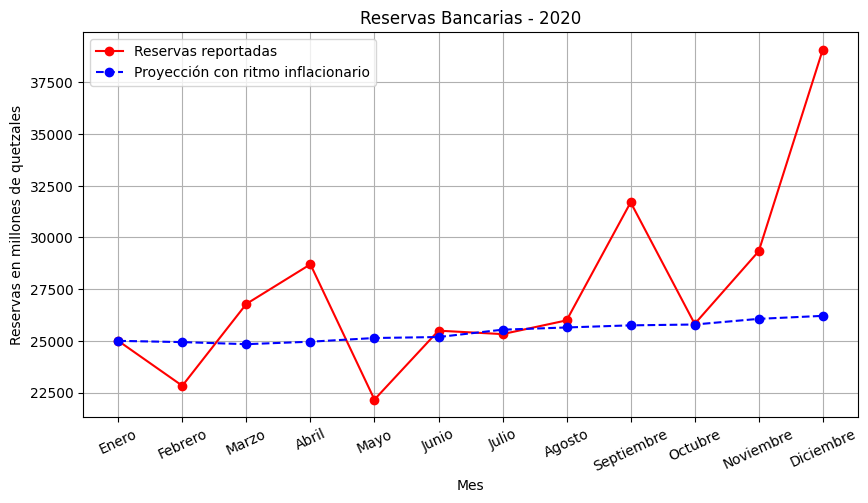
\includegraphics[width=\linewidth]{imagenes/reservas_2020.png}
    \caption{2020}
  \end{subfigure}
  % No hay espacio intencionalmente entre las figuras para maximizar el tamaño de la imagen
  \begin{subfigure}[b]{0.495\textwidth}
    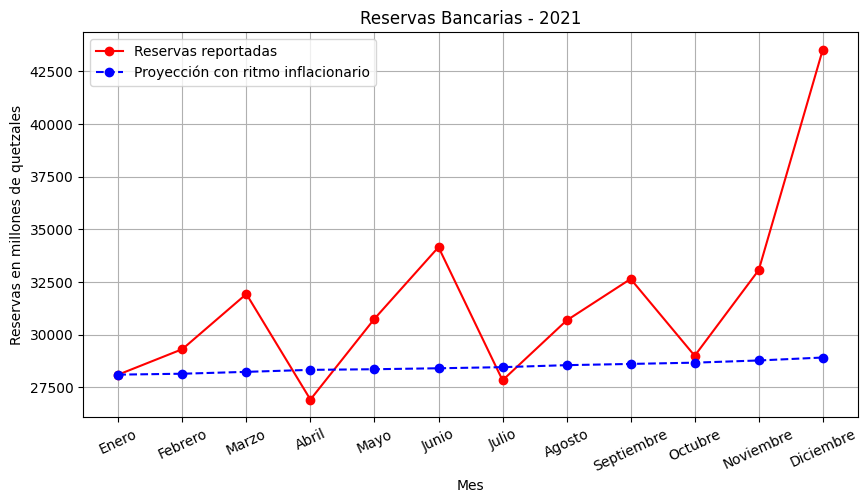
\includegraphics[width=\linewidth]{imagenes/reservas_2021.png}
    \caption{2021}
  \end{subfigure}
  
  % Fila 3
  \begin{subfigure}[b]{0.495\textwidth}
    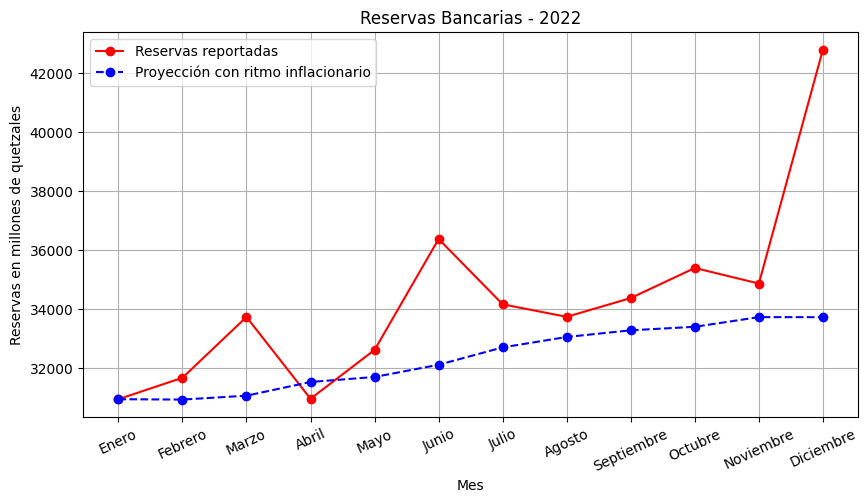
\includegraphics[width=\linewidth]{imagenes/reservas_2022.png}
    \caption{2022}
  \end{subfigure}
  % No hay espacio intencionalmente entre las figuras para maximizar el tamaño de la imagen
  \begin{subfigure}[b]{0.495\textwidth}
    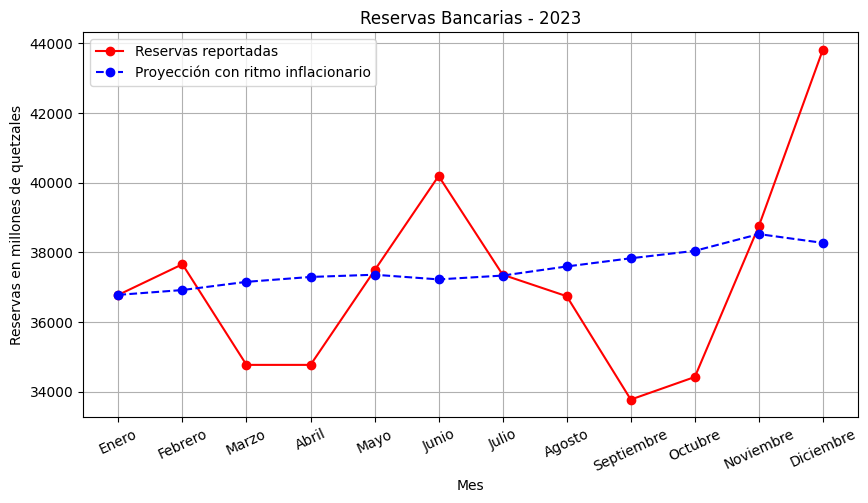
\includegraphics[width=\linewidth]{imagenes/reservas_2023.png}
    \caption{2023}
  \end{subfigure}
\caption{Proyección de valor constante de las Reservas a inicio de año bajo efecto de la inflación}
\end{figure}
\newpage
Observamos que las reservas proyectadas, que se ajustan por inflación de manera progresiva mes a mes, generalmente están por debajo de las reservas reales reportadas. Esto indica que las reservas bancarias no solo han crecido lo suficiente para contrarrestar la inflación, sino que han aumentado en términos de poder adquisitivo.
